\documentclass[11pt]{amsart}
\usepackage{geometry}                % See geometry.pdf to learn the layout options. There are lots.
\geometry{letterpaper}                   % ... or a4paper or a5paper or ... 
%\geometry{landscape}                % Activate for for rotated page geometry
%\usepackage[parfill]{parskip}    % Activate to begin paragraphs with an empty line rather than an indent
\usepackage{graphicx}
\usepackage{amssymb}
\usepackage{amsmath}
\usepackage{epstopdf}
\graphicspath{ {images/} }
\newtheorem{definition}{Definition}
\DeclareGraphicsRule{.tif}{png}{.png}{`convert #1 `dirname #1`/`basename #1 .tif`.png}

\title{Balancer: A protocol for multi-token automated market-making}
\author{Fernando Martinelli}
%\date{08/05/2019} % Activate to display a given date or no date

\begin{document}
\maketitle

\begin{abstract}
   Balancer is a new Ethereum-based protocol that allows any ERC20 portfolio to be continuously rebalanced while at the same time generating passive income through trading fees. Previously idle ERC20 tokens become Balancer pools, allowing anyone to trustlessly and non-custodially trade any two assets contained therein. Differently from Uniswap\footnote{https://uniswap.io/}, pools can contain any number of ERC20 tokens with arbitrary value weights. They are also owned and controlled individually, as opposed to combined into single pairwise markets like on Uniswap.
\end{abstract}

\section{Introduction}
%\subsection{}

Investment portfolios such as Index Funds are a very common financial instrument. The first index fund became effective in 1972, its investment objective being to approximate the performance of the Dow Jones Industrial Stock Average. Ever since, investors heavily rely on different portfolio strategies to hedge risk and achieve diversification. With blockchain, digital assets have become a new class of investment, which naturally ported the index fund concept from the conventional financial world to the new blockchain context. Index funds guarantee investors a constant and controlled exposure to a basket of assets. If one of its assets out- or under-performs, it is respectively sold or bought to keep its value share of the total portfolio constant.

Both in the conventional financial system as well as in the blockchain context, Index Funds and other types of investment portfolios charge investors fees for managing and holding their funds. These fees are necessary to pay for the costs of actively rebalancing the index funds, be it by manual traders or automatic bots. 

Balancer protocol, on the other hand, allows any portfolio owner to maintain their portfolio continuously and effortlessly rebalanced. This is done not only with the owner keeping full control and custody of their portfolio, but at the same time also being rewarded through trading fees, as we will see in detail in the following. 

To summarize, instead of paying fees to keep a balanced portfolio, ERC20 token holders can now earn fees by using Balancer protocol to do so. 


\section{Present Work}

There are many centralized solutions for portfolio management and for investing in index funds. We will however limit this analysis to the decentralized/non-custodial solutions in existence, since that is a fundamental characteristic Balancer protocol was designed to have.

Melonport\footnote{https://melonport.com/} is a protocol that allows fund managers to streamline and set up funds more easily than conventionally. Although an interesting concept, Melonport did not seem to get traction, as we believe it is still complicated to use and retail investors have to pay fees to participate in its investment funds. The existence of the MLN token also adds unnecessary friction to the process.

Set Protocol\footnote{https://www.tokensets.com/} is, in our view, a more interesting approach that has recently been launched and is gaining traction. It allows anyone to buy sets of tokens, i.e. tokens that represent ownership of a basket of other tokens. These sets may have embedded logic as for when the underlying tokens are swapped/exchanged for one another. For example, the 50\%/50\% BTC ETH set is a buy and hold strategy that rebalances monthly. Other more complex strategies include trend and range bound trading. 

It is important to stress that none of the protocols mentioned above provide liquidity providers with native rewards or earnings. On the contrary, rebalancing sets within Set Protocol incurs in both trading fees as well as network gas costs. The latter is currently being paid for by Set Labs Inc., the company that develops Set Protocol.

Uniswap, Kyber\footnote{https://kyber.network}  and Compound\footnote{https://compound.finance/} are examples of protocols that enable liquidity providers to earn fees through providing liquidity.

Balancer Protocol achieves the objective of rebalancing portfolios as does Set Protocol at the same time rewarding liquidity providers as does Uniswap. Balancer is a generalization of Uniswap. All Uniswap exchanges can be emulated with Balancer Protocol, however the opposite is not true: arbitrary portfolios cannot be invested and continuously rebalanced in Uniswap as they can with Balancer Protocol. 

\section{Balancer Protocol Architecture}
\subsection{Balancer Pools}
Balancer pools are the building blocks of Balancer protocol. Any Ethereum address that owns two or more ERC20 tokens can create a Balancer Pool, as illustrated in Figure \ref{fig:example_balancer_pool}.

\begin{figure}
  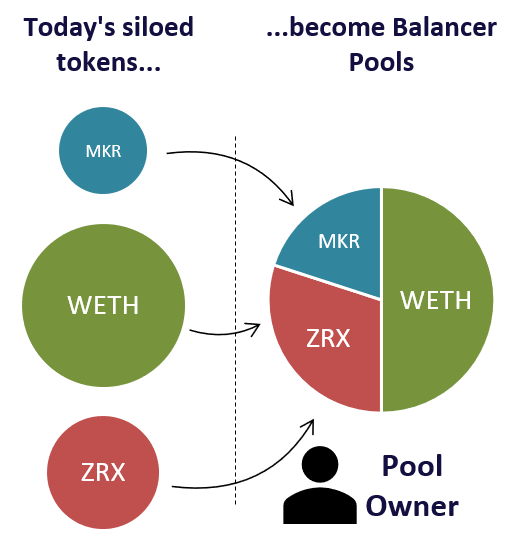
\includegraphics[]{example_balancer_pool}
  \caption{Example of Balancer Pool containing a value distribution of 50\% in WETH, 30\% in ZRX and 20\% in MKR tokens.}
  \label{fig:example_balancer_pool}
\end{figure}

The pool will have a certain total value and each of the tokens will make up a percentage of that value. These percentages are the token weights. These weights are defined upon the pool creation and can be changed at any later time by the pool owner. If not changed, Balancer Protocol will ensure that the percentage of value each token in the pool represents will remain stable, even if exchange rates between tokens may change. This is achieved through protocol incentives created for arbitrageurs to arbitrage between Balancer pools and external markets---other centralized or decentralized exchanges. 

\subsection{Trading with Individual Pool}
Balancer Pools are automated market-makers because they allow any Ethereum user to trade on any pair contained in the pool. In the example pool above one could trade on any of the following pairs: WETH/MKR, MKR/ZRX and ZRX/WETH. Both directions, buying or selling, are always possible.

\subsubsection{Spot Exchange Rate}
Similarly to Uniswap, we propose the exchange rates of any of the $\frac{(n^2 - n)}{2}$ pairs of tokens within a pool of $n$ tokens to be defined exclusively by their balances\footnote{This means that the system state and its evolution is self-contained, i.e. no external feeds or oracles are necessary. This makes Balancer Protocol an excellent and trustworthy oracle, so long as there is enough liquidity available.}. We propose nevertheless an addition that enables Balancer pools to assume any basket value distribution as opposed to Uniswap\footnote{In Uniswap each exchange pair always holds the same value in ETH as in the ERC20 token. This is a consequence of the simple invariant function $x.y=k$ used, where $x$ represents the ETH balance, $y$ represents the ERC20 balance and $k$ is a value that would remain constant after any number of trades, were it not for the 0.3\% fees charged.}. The spot exchange rate between any two tokens, $SpotExchangeRate^{o}_{i}$, or in short $SER^{o}_{i}$, is the the ratio of the token balances \textit{normalized} by their weights:

\begin{equation}
\label{equation:SER}
SER^{o}_{i} = \frac{\frac{B_{o}}{W_{o}}}{\frac{B_{i}}{W_{i}}}
\end{equation}

Where:
\begin{itemize}
    \item $B_{o}$ is the balance of token \textit{o}, the token being bought by the trader which is going \textit{out} of the pool.
    \item $B_{i}$ is the balance of token \textit{i}, the token being sold by the trader which is going \textit{into} the pool.
    \item $W_{o}$ is the weight of token \textit{o}
    \item $W_{i}$ is the weight of token \textit{i}

\end{itemize}

For example, if in the pool described above we had 10 WETH, 6000 ZRX and 1 MKR, then the spot exchange rates offered by this pool would be:

\begin{align*}
SER^{W}_{M} = \frac{\frac{B_{W}}{W_{W}}}{\frac{B_{M}}{W_{M}}} = \frac{\frac{10}{0.5}}{\frac{1}{0.2}} = 4  \end{align*}

\begin{align*}
SER^{M}_{Z} = \frac{\frac{B_{M}}{W_{M}}}{\frac{B_{Z}}{W_{Z}}} = \frac{\frac{1}{0.2}}{\frac{6000}{0.3}} = 0.00025
\end{align*}

\begin{align*}
SER^{Z}_{W} = \frac{\frac{B_{Z}}{W_{Z}}}{\frac{B_{W}}{W_{W}}} = \frac{\frac{6000}{0.3}}{\frac{10}{0.5}} = 1000 \end{align*}

The spot exchange rate in the opposite direction of the trade is just the inverse of the original:

\begin{equation}
SER^{i}_{o} = \frac{1}{SER^{o}_{i}}
\end{equation}

\subsubsection{Effective Exchange Rate}

It is important to bear in mind that $SER^{o}_{i}$ is the theoretical exchange rate for infinitesimal trades, which would incur in no slippage. In practice, the effective exchange rate for any trade depends on the amount being traded, which always leads to some slippage. If we define $A_{o}$ as the amount of token $o$ being bought by the trader and $A_{i}$ as the amount of token $i$ being sold by the trader, then we can define $EffectiveExchangeRate^{o}_{i}$, or in short $EER^{o}_{i}$ as:

\begin{equation}
EER^{o}_{i} = \frac{A_{o}}{A_{i}} \end{equation}

And as mentioned above, $EER$ tends to $SER$ when traded amounts tend to 0:

\begin{equation}
\label{equation:EER_tends_to_SER}
SER^{o}_{i} = \lim_{A_{o},A_{i}\to 0} EER^{o}_{i}
\end{equation}

The derivation of $A_{o}$ in terms of $A_{i}$ and vice-versa depend on the multidimensional invariant surface described in detail in section \ref{section:maths}.

\subsubsection{Arbitrage and External Market Exchange Rate Matching}
From Eq.\ref{equation:SER}, considering weights constant during trades\footnote{Weights can be changed at any time by the pool owner. However since trade events are atomic, weights cannot be changed by the pool owner during a trade.}, the spot exchange rates offered by Balancer Pools only change with changing token balances. If the pool owner does not add or remove tokens to/from the pool, token balances can only change through trades. We have then a feedback loop that causes exchange rates of tokens being bought (token $o$) to decrease---i.e their prices increase---and vice-versa. One can prove that whenever external market exchange rates are different from those offered by a Balancer Pool, an arbitrageur will make the most profit by trading with that pool until its exchange rates equal those on the external market. When this happens there is no more arbitrage opportunity. These arbitrage opportunities are the reason why we see Uniswap exchange rates move in lockstep with the rest of the market.

\subsection{Off-Chain Smart Order Routing (SOR)}
Since Balancer Protocol allows any number of pools to be created, there may be several different pools that contain any given trading pair. If a trader wants to trade 100 Token A for Token B and the whole trade is carried out only in a single Balancer Pool, there may be a lot of slippage. That slippage would create a difference between exchange rates amongst different Balancer Pools, allowing for arbitrageurs to profit. In other words, trading with only one pool is equivalent to leaving money on the table only for arbitrageurs.

A better approach to minimize slippage and maximize the amount of tokens B received is spreading the 100 Tokens A across multiple Balancer pools such that all trades shift the exchange rates of the pools to the same value. Finding which amounts should be traded and in what pools is a non-linear, multi-variable optimization problem. Balancerpro.com has a free off-chain Smart Order Routing algorithm that solves this problem and finds the exact amounts to be traded with the most advantageous pools available. For that optimization we take into account the gas price selected as well as the states of all available Balancer pools in the desired pair. Fig.\ref{fig:smart_order_routing} illustrates an example of the Smart Order Routing process.

\begin{figure}
  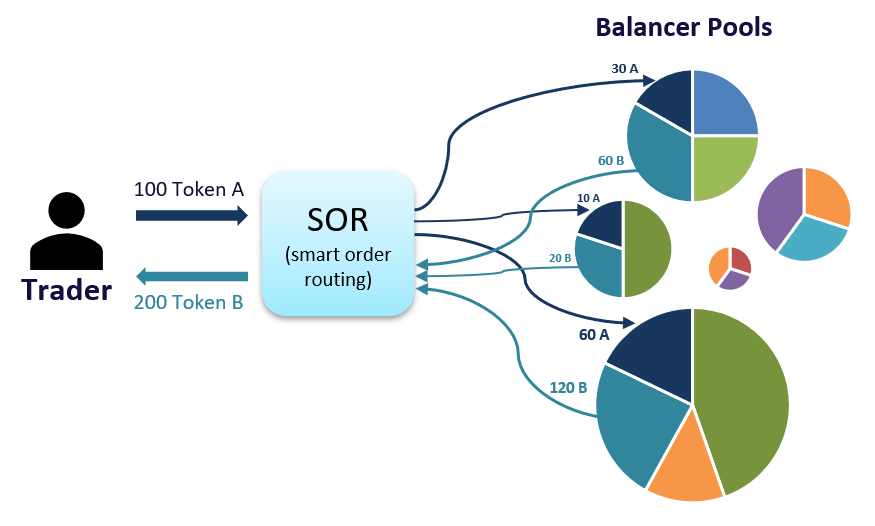
\includegraphics[]{smart_order_routing}
  \caption{Example of trade using Balancer's smart order routing to maximize returns.}
  \label{fig:smart_order_routing}
\end{figure}

\section{Mathematical Background and Proofs}
\label{section:maths}

\subsection{Value function}
The bedrock of Balancer Protocol's mathematical framework is a value function that, when kept invariant, ensures that the spot exchange rates of any two tokens are as defined in Eq.\ref{equation:SER}. As we will see in section \ref{section:proof_constant_value_distribution}, this property has as corollary that the value distribution across all tokens is kept constant. This is what makes Balancer Protocol suitable for rebalancing portfolios.

We propose $V$ to be defined as:
\begin{equation}
\label{equation:value_function}
V = \prod_{k}(B_k)^{W_k}
\end{equation}

with:

\begin{equation}
\label{equation:sum_weights}
\sum_{k} W_k = 1
\end{equation}

The value function goes strictly up with the fees charged by Balancer Pools for each trade. However, for simplicity's sake, let's assume no fees are charged and we enforce that the value function remain constant. In other words, we make $V$ an invariant.

\subsection{Spot Exchange Rate proof}
Let's now prove that this choice of $V$ entails Eq.\ref{equation:SER}.

First of all, we know that what the trader buys, $A_{o}$, is subtracted from the contract's balance. Therefore $A_{o}=-\Delta B_{o}$. Likewise, what the trader sells, $A_{i}$, is added to the contract's balance. Therefore $A_{i} = \Delta B_{i}$.

Substituting in Eq.\ref{equation:EER_tends_to_SER} we get:

\begin{equation}
\label{equation:proof_partial_derivative_1}
SER^{o}_{i} = \lim_{A_{o},A_{i}\to 0} EER^{o}_{i} = \lim_{\Delta B_{o},\Delta B_{i}\to 0} \frac{-\Delta B_{o}}{\Delta B_{i}}
\end{equation}

This limit is, by definition, minus the partial derivative of $B_{o}$ in function of $B_{i}$:

\begin{equation}
\label{equation:proof_partial_derivative_2}
SER^{o}_{i} = -\frac{\partial B_{o}}{\partial B_{i}}
\end{equation}

From the value function definition in Eq.\ref{equation:value_function} we can isolate $B_{o}$:

\begin{equation}
\label{equation:proof_partial_derivative_3}
\begin{gathered}
(B_{o})^{W_{o}} =  \frac{V}{\left(\prod_{k\neq out, k\neq in}(B_k)^{W_k}\right).(B_{i})^{W_{i}}}\\
B_{o} =  \left(\frac{V}{\left(\prod_{k\neq out, k\neq in}(B_k)^{W_k}\right).(B_{i})^{W_{i}}}\right)^\frac{1}{W_{o}}
\end{gathered}
\end{equation}

Now we use Eq.\ref{equation:proof_partial_derivative_3} to expand the partial derivative in Eq.\ref{equation:proof_partial_derivative_2}:

\begin{equation}
\begin{gathered}
SER^{o}_{i} =
-\frac{\partial B_{o}}{\partial B_{i}} =
-\frac{\partial{\left(\left(\frac{V}{\left(\prod_{k\neq out, k\neq in}(B_k)^{W_k}\right).(B_{i})^{W_{i}}}\right)^\frac{1}{W_{o}}\right)}}{\partial B_{i}}  =\\
=-\left(\frac{V}{\prod_{k\neq out, k\neq in}(B_k)^{W_k}}\right)^\frac{1}{W_{o}}
.
\frac{\partial{\left(B_{i}^{-\frac{W_{i}}{W_{o}}}\right)}}{\partial B_{i}} =\\
=-\left(\frac{V}{\prod_{k\neq out, k\neq in}(B_k)^{W_k}}\right)^\frac{1}{W_{o}}
.
-\frac{W_{i}}{W_{o}}.B_{i}^{-\frac{W_{i}}{W_{o}}-1} =\\
=\left(\frac{V}{\prod_{k}(B_k)^{W_k}}\right)^\frac{1}{W_{o}}
.B_{i}^{\frac{W_{i}}{W_{o}}}.B_{o}
.\frac{W_{i}}{W_{o}}.B_{i}^{-\frac{W_{i}}{W_{o}}-1} = \frac{\frac{B_{o}}{W_{o}}}{\frac{B_{i}}{W_{i}}}
\end{gathered}
\end{equation}

which concludes our proof.

\subsection{Constant Value Distribution Proof}
\label{section:proof_constant_value_distribution}
We will now prove that:
\begin{enumerate}
    \item Balancer Pools maintain a constant share of value across all tokens in the pool and;
    \item These shares of value are equal to the weights associated to each token.
\end{enumerate}

Let's calculate $V^1$, the total pool value in terms of token $1$---it can really be any token in the pool since they are not necessarily ordered. Since we already know that the pool has $B_1$ tokens $1$, let's calculate how many tokens $1$ all the other remaining tokens are worth. It does not make sense to use their Effective Exchange Rate relative to token $1$ since we are not going to do any actual trade. Instead, to calculate the theoretical value we use their Spot Exchange Rates relative to token $1$.

From Eq.\ref{equation:SER} we can calculate $V^1_n$, i.e how many tokens $1$ the balance of each token $n$ is worth:
\begin{equation}
\label{equation:value_i_tokens1}
V^1_n = B_{n} . SER^{1}_{n} = B_{n} . \frac{\frac{B_{1}}{W_{1}}}{\frac{B_{n}}{W_{n}}} =
B_{1}.\frac{W_{n}}{W_{1}}
\end{equation}

We know that the total pool value in terms of tokens $1$ is the sum of the values of each token in terms of tokens $1$:

\begin{equation}
\label{equation:total_value_i_tokens1}
V^1 = \sum_{k}V^1_k = B_{1} +\sum_{k\neq 1}V^1_k =
B_{1} + \frac{B_{1}}{W_{1}}.\sum_{k\neq 1}W_n =
\frac{B_{1}}{W_{1}}.(W_1+\sum_{k\neq 1}W_n) = \frac{B_{1}}{W_{1}}
\end{equation}

Now to calculate $S_n$, the share of value each token represents in the pool, all we have to do is divide the value of each token $V^1_n$ by the total pool value $V^1$:

\begin{equation}
\label{equation:total_value_i_tokens1}
S_n = \frac{V^1_n}{V^1} = W_n
\end{equation}

which proves both that the share each token represents of the total pool value is constant and also that it is equal to the weight of that token.


\section{Trading Formulae}

Calculating the trade outcomes for any given Balancer Pool is easy if we bear in mind that the Value Function $V$ must remain invariant\footnote{Again, this is a simplification for a Balancer Pool that does not charge any fees for trades, in practice trades are charged a fee that causes the value function to strictly increase}, i.e. $V$ must have the same value before and after any trade.

\subsection{Amount of Token $o$ for Given Amount of Token $i$}
When a user sends tokens $i$ to get tokens $o$, all other token balances remain the same. Therefore, if we define $A_{i}$ and $A_{o}$ as the amount of tokens $i$ and $o$ exchanged, we can calculate the amount $A_{o}$ a users gets when sending $A_{i}$:

\begin{equation}
\label{equation:A_o}
\begin{gathered}
(B_{o}-A_{o})^{W_{o}}.(B_{i}+A_{i})^{W_{i}} = B_{o}^{W_{o}}.B_{i}^{W_{i}} \\
B_{o}-A_{o} = \frac{B_{i}^{\frac{W_{i}}{W_{o}}}.B_{o}}{(B_{i}+A_{i})^{\frac{W_{i}}{W_{o}}}}\\
A_{o} = \left(1 - \left(\frac{B_{i}}{B_{i}+A_{i}}\right)^{\frac{W_{i}}{W_{o}}}\right).B_{o}
\end{gathered}
\end{equation}

\subsection{Amount of Token $i$ for Given Amount of Token $o$}
It is also very useful for traders to know how much they need to send of the input token $A_{i}$ to get a desired amount of output token $A_{o}$. We can calculate the amount $A_{i}$ as a function of $A_{o}$ similarly as follows:

\begin{equation}
\begin{gathered}
(B_{o}-A_{o})^{W_{o}}.(B_{i}+A_{i})^{W_{i}} = B_{o}^{W_{o}}.B_{i}^{W_{i}} \\
B_{i}+A_{i} = \frac{B_{o}^{\frac{W_{o}}{W_{i}}}.B_{i}}{(B_{o}-A_{o})^{\frac{W_{o}}{W_{i}}}}\\
A_{i} = \left(\left(\frac{B_{o}}{B_{o}-A_{o}}\right)^{\frac{W_{o}}{W_{i}}}-1\right).B_{i}
\end{gathered}
\end{equation}

Notice that $A_{o}$ as defined by Eq.\ref{equation:A_o} tends to $SER^{o}_{i}.A_{i}$ when $A_{i} << B_{i}$, as expected. This can be proved by using L'Hopital's rule\footnote{https://en.wikipedia.org/wiki/L'Hopital's\_rule} but this proof is out of the scope of this paper.

\subsection{Amount of Token $i$ to New Desired Spot Exchange Rate}
For practical purposes, traders intending to use our contract for arbitrage will like to know what amount of tokens $i$ -- $A_{i}$ -- they will have to send to the contract to change the current spot exchange rate $SER^{o}_{i}$ to another desired one $SER^{o}_{i}'$. The desired spot exchange rate will usually be the external market exchange rate and, so long as the contract spot exchange rate differs from the external market's, any arbitrageur can profit by trading with the contract and bringing the contract exchange rate closer to the external market's.

The highest profit possible by an arbitrageur is when they bring the contract spot exchange rate exactly to the external market's exchange rate. As already mentioned, this is the main reason why our design is successful in keeping track of the market prices, thus being a reliable on-chain price sensor.

It can be proved with a little math effort, which we consider out of this paper's scope, that the amount of tokens $i$ -- $A_{i}$ -- a user needs to trade against tokens $o$ so that the pool's spot exchange rate changes from $SER^{o}_{i}$ to $SER^{o}_{i}'$ is:

\begin{equation}
\begin{gathered}
A_{i} = \left(\left(\frac{SER^{o}_{i}}{SER^{o}_{i}'}\right)^\frac{W_{o}}{W_{o}+W_{i}} - 1 \right).B_{i}
\end{gathered}
\end{equation}

\section{Specifications and Smart Contract Design}

\subsection{Overview}
Here we show the main smart contracts in the system and how each actor can interact with them: pool owners can set pool balances, weights and fees; traders can swap any pair of tokens directly with one or many pools (for example using SOR).

\subsection{Functions (maybe for appendix?)}
Details of input and returned params

\subsection{ERC20 Standard Considerations}
See this section in Set Protocol's paper: https://www.setprotocol.com/pdf/set\_protocol\_whitepaper.pdf
Interesting for us as well: 
- Variant ERC20 Decimals
- Variant Transfer Receive Quantities
- Variant Transfer Return Values


\section{References}
Whitepapers, Vitalik's post about x*y = k etc.

\end{document}  